The United States has been the forerunner in nuclear energy, with a currently 
installed nuclear capacity of 99,221 \gls{MWe} \cite{iaea_nuclear_2017}.
With its large capacity and long history of nuclear
energy, the United States has accumulated over $70,000$ \gls{MTHM} of \gls{UNF}.

The challenge with modeling the U.S. transition scenario is that the U.S. does not have
a single nationwide advanced reactor vision, whereas France has a central plan to transition into \gls{ASTRID} reactors \cite{boullis_french_2015, varaine_pre-conceptual_2012}.
Previous analyses of the United States \cite{worrall_utilization_2013, sunny_transition_2015}
 \gls{NFC} transition scenario
assumed transition to fast-spectrum \glspl{SFR}.
However, the fact that the U.S. nuclear reactor fleet
is decided by economic interests (industries), necessitates
exploration of different options, such as transitioning into \glspl{MSR}.

As explained in section \ref{sec:msr}, rising interests in \gls{MSR} designs
led to a proliferation of U.S. corporations aiming to commercialize
\gls{MSR} designs. Given the large interest from industries,
\gls{MSR} designs are
most likely to be commercially deployed in the United States.

In this chapter, I explore the U.S. transition scenario
from an \gls{LWR} fleet into an \gls{MSR} fleet.

\section{Initial conditions and scenario parameters}

For the French scenario, the \gls{UNF} inventory at the present
time is calculated by simulating the nuclear operational history from 1970.
However, this is unnecessary for the U.S. scenario because a detailed
database exists that describes the U.S. \gls{UNF} inventory up to May of 2013.
The \gls{UNF-STANDARDS} is a comprehensive,
controlled source of \gls{UNF} information, including dry cask attributes, assembly
data, and economic attributes \cite{peterson_unf-st&dards_2017}. The assembly
compositions are calculated using ORIGEN \cite{parks_overview_1992} using the
reported fuel assembly burnups, original enrichment, and assembly design. This database
allows the transition scenario simulation to start from 2013. I imported 
the \gls{UNF} inventory mass and composition in 2013
from \gls{UNF-STANDARDS} and `initiated' the inventory in the simulation
as a \texttt{Source} facility with an inventory of 68,072 MTHM,
the total mass of the \gls{LWR} \gls{UNF} in the \gls{UNF-STANDARDS}.

Furthermore, the U.S. currently has additional uranium resources in the
form of more than $700,000$ MTHM of depleted uranium \cite{office_nuclear_2011},
which is a waste product of enrichment. The depleted uranium inventory
is currently a liability and waste, but can be utilized as fertile material
in a U-Pu fuel cycle. If the U.S. chooses a Th-$^{233}U$ fuel cycle,
additional thorium resources are needed, while with a U-Pu cycle, the
U.S. can use its waste to create fuel.

The U.S. nuclear fleet in 2013 can be extracted from the \gls{PRIS} database.
The same assumption that legacy reactors have a 60-year lifetime is applied
to calculate the remaining lifetime of legacy reactors.
I used \texttt{from\_pris} to generate the expected power capacity
of the current U.S. nuclear from 2013 (shown in figure \ref{fig:us_legacy}).

\begin{figure}[htbp!]
	\begin{center}
		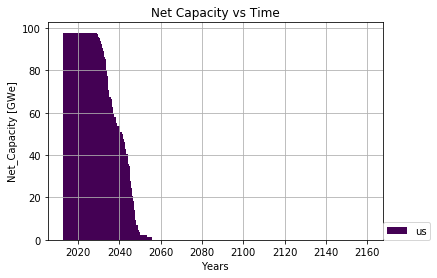
\includegraphics[scale=0.7]{./images/us/legacy_power.png}
	\end{center}
	\caption{Installed nuclear capacity in the United States from 2013.}
	\label{fig:us_legacy}
\end{figure}


\subsection{Energy Demand Prediction}
A reference for the energy demand prediction is the 
\gls{EIA} Annual Energy Outlook \cite{u.s._eia_annual_2018}.
The 2018 Annual Energy Outlook report predicts an annual electricity demand growth
of 0.9\%. The report also predicts that nuclear
power will either remain static or decrease. The report
predicts that nuclear capacity will decrease from 99 GWe
to 79GWe in 2050, with no new plants beyond 2020.
However, for this work,
I assume that the U.S. nuclear power capacity is kept at
100GWe, and new reactors are deployed to make up for the
decommissioned capacity.

\subsection{\gls{MSR} Design and Availability}

\gls{MSR} designs can be categorized depending on their operating
neutron spectrum (e.g. fast, thermal), fuel cycle (e.g. Th-$^{233}U$, U-Pu),
and transmutation goals (e.g. breeder, burner). Selection of an \gls{MSR}
design depends on factors like economics, safety, and fuel cycle
considerations. For this work, I choose a fast, U-Pu cycle, burner \gls{MSR} design
named REBUS-3700 \cite{mourogov_potentialities_2006} to deploy for the
transition analysis.

The REBUS-3700 \gls{MSR} design offers five principal
advantages over other \gls{MSR} designs:
\begin{itemize}
	\item Fast spectrum - no need for moderator rods
	\item U-Pu cycle - requires only depleted uranium for supply after initial fuel salt loading
	\item Weakly positive breeding gain (0.03)
	\begin{itemize}
		\item Self-sufficient (no external fissile input)
		\item No surplus fissile material production (stabilizes Pu inventory)
	\end{itemize}
	\item U-\gls{TRU} initial fuel - transmutation of long-lived actinides
	\item Simpler design - no radial / axial blanket
\end{itemize}

The U.S. has a large inventory of \gls{LWR} \gls{UNF} and tails. The benefits
of the REBUS-3700 design aligns with the waste management interest
of the U.S. Reducing final geological repository burden can be
accomplished by:

\begin{itemize}
	\item Reduction of \gls{TRU} inventory by transmutation in the reactor (table \ref{tab:rebus_comp})
	\begin{itemize}
		\item Reduction of long-term decay heat and activity (figure \ref{fig:decay_heat})
		\item More `tailored' waste form design for fission products
	\end{itemize}
	\item Reducing tails inventory
\end{itemize}

Additionally, the REBUS-3700 does not have, at any moment in
operation, separated fissile streams, like other \gls{MSR} designs.
Other \gls{MSR} designs such as the
\gls{MCSFR} design \cite{smith_assessment_1974}
have separated fissile streams, since it separates the bred plutonium from its blanket salt.
The REBUS-3700 only takes in depleted uranium and processes out
fission product groups such as volatile gases and noble metals.
The detailed reprocessing scheme is shown
in table \ref{tab:rebus_reproc}. 
This self-sustained and closed operation increases its non-proliferation
properties.

The initial fuel and equilibrium \gls{TRU} isotopic composition of REBUS-3700 is
shown in table \ref{tab:rebus_comp}. The \gls{TRU} isotopic composition
matches that of the \gls{LWR} \gls{UNF} after 8.5 years of decay (shown
in figure \ref{fig:trutru}).


\begin{figure}[htbp!]
	\begin{center}
		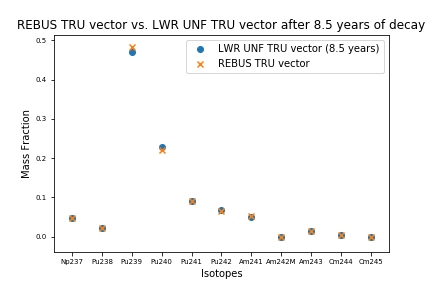
\includegraphics[scale=0.7]{./images/us/trutru.png}
	\end{center}
	\caption{\gls{TRU} vector of REBUS-3700 initial fuel from Mourogov et al. \cite{mourogov_potentialities_2006}
		with \gls{LWR} \gls{UNF} after 51 GWdth/MTHM burnup and 8.5 years of decay}
	\label{fig:trutru}
\end{figure}


\begin{table}[h]
	\centering
	\caption{Initial and equilibrium \gls{TRU} isotopic composition from Mourogov et al. \cite{mourogov_potentialities_2006}.}
	\label{tab:rebus_comp}
	\begin{tabularx}{\textwidth}{lll}
		\hline
		Isotope & Beginning of Life & Equilibrium (\textasciitilde 6500 \gls{EFPD}) \\
		\hline
		$^{237} Np$ / $^{239} Np$ &  4.80 / 0.00 & 0.65 / 0.07 \\
		$^{238} Pu$ / $^{239} Pu$ & 2.13 / 48.33  & 2.23 / 58.02  \\
		$^{240} Pu$ / $^{241} Pu$ / $^{242} Pu$ & 22.17 / 9.05 / 6.38 & 27.63 / 3.35 / 4.05 \\
		$^{241} Am$ / $^{242m} Am$ / $^{243} Am$ &5.17 / 0.01 / 1.48 & 1.50 / 0.12 / 1.05 \\
		$^{242} Cm$ / $^{243} Cm$  & 0.0 /0.0  & 0.07 / 0.01  \\
		$^{244} Cm$ / $^{245} Cm$ / $^{246} Cm$ & 0.43 / 0.04 / 0.00 & 1.02 / 0.19 / 0.05 \\
		Equivalent enrichment, \% & 10.1 & 11.0 \\
		\gls{TRU} fraction in heavy atoms, \% & 15.6 & 15.9 \\
		\hline
	\end{tabularx}
\end{table}


\begin{table}[h]
	\centering
	\caption{Reprocessing scheme for REBUS-3700}
	\label{tab:rebus_reproc}
	\begin{tabular}{lll}
		\hline
		Group & Elements & Reprocessing Time (s) \\
		\hline
		Volatile Gases & Kr, Xe, Ar, Ne, H, N, O, Rn & 30 \\
		Noble Metals & \shortstack{Se, Nb, Mo, Tc, Ru, Rh,\\ Pd, Ag, Sb, Te, Zr, Cd, In, Sn} & 30 \\
		Rare Earths & \shortstack{Y, La, Ce, Pr, Nd, Pm, Sm, Gd, \\ Eu, Dy, Ho, Er, Tb, Ga, Ge, As, Zn} & 259,200 \\
		\hline
	\end{tabular}
\end{table}



\section{U.S. deployment schedule}

As shown in figure \ref{fig:us_legacy}, the U.S. will
undergo a profound loss of nuclear capacity from 2030, under the
assumption that U.S. reactors have a lifetime of 60 years.

Since it is unlikely that \glspl{MSR} are ready for
commercial deployment in 2020, I deploy \glspl{LWR} (AP 1000 design \cite{sutharshan_ap1000tm_2011})
to make up for the decommissioned capacity in the simulation. After 2050,
REBUS-3700 design \glspl{MSR} are deployed. The deployment of new reactors
is shown in figure \ref{fig:us_dep}, and the installed
power capacity of the reactors is shown in \ref{fig:us_pow}.
In the simulation, 84 additional \glspl{LWR} and 95 \glspl{MSR}
are deployed.

\begin{figure}[htbp!]
	\begin{center}
		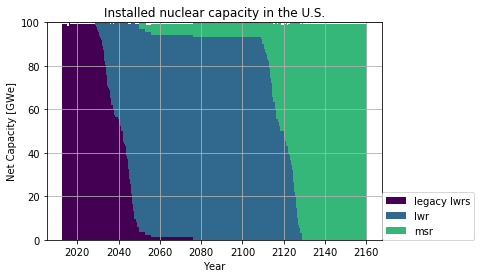
\includegraphics[scale=0.7]{./images/us/power_plot.png}
	\end{center}
	\caption{Power capacity separated by reactor type from 2020.}
	\label{fig:us_pow}
\end{figure}

\begin{figure}[htbp!]
	\begin{center}
		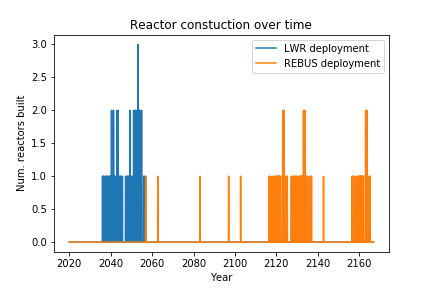
\includegraphics[scale=0.7]{./images/us/us_dep.png}
	\end{center}
	\caption{New reactor deployment from 2020.}
	\label{fig:us_dep}
\end{figure}

\section{Material flow}

The fuel cycle is represented by a series of facility agents whose material 
flow is illustrated in figure \ref{diag:us_fc}, along with
the \Cyclus archetypes that were used to model each facility.

\begin{figure}
	\centering
	\scalebox{0.6}{
		\begin{tikzpicture}[align=center, node distance = 3cm and 3cm, auto]
		% Place nodes
		\node [block] (sr) {Mine (\texttt{SOURCE})};
		\node [cloud, below of=sr] (nu) {Nat U};
		\node [block, below of=nu] (enr) {\small Enrichment ({\scriptsize \texttt{ENRICHMENT}})};
		\node [cloud, below of=enr] (uox) {\acrshort{UOX}};
		\node [block, below of=uox] (lwr) {\gls{LWR} (\texttt{REACTOR})};
		\node [cloud, right of=lwr] (snf) {\gls{UNF}};
		\node [block, right of=snf] (pool) {Pool (\texttt{Storage})};
		\node [cloud, left of=uox] (tl2) {Dep U};
		\node [block, below of=tl2] (stor) {Storage (\texttt{Storage})};
		\node [block, right of=tl] (sk) {Repository (\texttt{SINK})};
		\node [cloud, below of=sk] (cunf) {Cooled \gls{UNF}};
		\node [cloud, below of=pool] (cunf2) {Cooled \gls{UNF}};
		\node [block, below of=snf] (rep) {{\footnotesize Reprocessing ({\scriptsize \texttt{SEPARATIONS}})}};
		\node [cloud, below of=rep] (u) {Sep. U} ;
		\node [cloud, left of=rep] (pu) {Sep. TRU};
		\node [block, left of=pu] (mix) {Fabrication (\texttt{MIXER})};
		\node [cloud, below of=mix] (fs) {Fuel Salt};
		\node [block, below of=mox] (mxr) {\gls{MSR} (\small \texttt{SaltProc-} \\ \texttt{Reactor})};
		\node [cloud, left of=stor] (tl) {Dep U};
		
		\node [cloud, right of=mxr] (waste) {Waste};
		\node [cloud, below of=waste] (eols) {End-of-life salt};
		
		\draw[->, thick] (sr) -- (nu);
		\draw[->, thick] (nu) -- (enr);
		\draw[->, thick] (enr) -- (tl2);
		\draw[->, thick] (tl2) -- (stor);
		\draw[->, thick] (enr) -- (uox);
		\draw[->, thick] (uox) -- (lwr);
		\draw[->, thick] (lwr) -- (snf);
		
		\draw[->, thick] (lwr) -- (snf);
		\draw[->, thick] (snf) -- (pool);
		\draw[->, thick] (pool) -- (cunf);
		\draw[->, thick] (pool) -- (cunf2);
		\draw[->, thick] (cunf) -- (sk);
		\draw[->, thick] (cunf2) -- (rep);
		
		\draw[->, thick] (rep) -- (u);
		\draw[->, thick] (rep) -- (pu);
		\draw[->, thick] (pu) -- (mix);
		\draw[->, thick] (mix) -- (mox);
		\draw[->, thick] (mox) -- (mxr);
		
		\draw[->, thick] (stor) -- (tl);
		\draw[->, thick] (tl) to [bend right] (mxr);
		\draw[->, thick] (tl) -- (mix);
		\draw[->, thick] (nu) -- node{} ++ (-8cm, 0) |- (mix) ;
			
		\draw[->, thick] (mxr) -- (waste);
		\draw[->, thick] (waste) to [bend right=80] (sk);
		\draw[->, thick] (mxr) -- (eols);
		\draw[->, thick] (eols) to [bend right=80] (sk);		
		
		\end{tikzpicture}
		
	}
	\caption{Fuel cycle facilities (blue boxes) represented by 
		\Cyclus archetypes (in parentheses) pass materials (red 
		ovals) around the simulation.} 
	\label{diag:us_fc}
\end{figure}

The U.S. transition scenario's material flow is similar to that of the French transition
in the previous chapter,
except that all \gls{TRU} is reprocessed from \gls{LWR} \gls{UNF}
to fabricate fuel salt. Also, the depleted uranium from
the enrichment plant is stored in a storage facility to be used as a fertile stream for \gls{MSR} facilities.
Natural uranium is mixed with the reprocessed \gls{TRU} to create fuel salt.
Lastly, instead of a single
stream of \gls{MOX} \gls{UNF} from the \gls{MOX} reactors, \glspl{MSR}
output two streams - reprocess waste and end-of-life salt - which are both disposed.

\FloatBarrier


\section{Scenario specification}

The scenario specifications for the U.S. transition scenario are listed
in table \ref{tab:us_sim_specs}.

\begin{table}[h]
	\centering
	\caption{Simulation Specifications}
	\begin{tabularx}{\linewidth}{bqq}
		\hline
		\textbf{Specification} &\textbf{ Value} & \textbf{Units}\\
		\hline
		Simulation Starts & 2013 & year\\
		Simulation Ends & 2160 & year\\
		Production of \gls{MSR} fuel begins & 2030 & year\\
		\glspl{MSR} become available & 2050 & year\\
		Reprocessed uranium usage &  None & -\\
		Minimum \gls{UNF} cooling time  & 8.5  & years\\
		Separation efficiency of \gls{TRU} and U & 99.8 & \% \\
		Reprocessing streams & Am, Pu, Cm, Np and U & - \\
		Reprocessing capacity & $\infty$ & \gls{MTHM}/month\\
		\gls{MSR} fuel salt fabrication throughput & No limit ($\infty$) & \gls{MTHM}/month \\
		\hline
	\end{tabularx}
	\label{tab:us_sim_specs}
\end{table}

\section{Reactor specifications}

Two major reactors are used in the simulation, \gls{PWR} and \gls{MSR}.

For \glspl{PWR}, I use a linear core size model to capture varying reactor capacity
(explained in section \ref{sec:writeinput}). The reactors deployed after 2020 are
modeled after the AP-1000 reactor \cite{sutharshan_ap1000tm_2011}. The reactor
specifications are shown in \ref{tab:us-reactor-specs}.

\begin{table}[h]
	\centering
	\caption{Baseline \gls{LWR} and \gls{MSR} simulation specifications.}
	\begin{tabular}{lrr}
		\hline
		\textbf{Specification} & \textbf{\gls{PWR} \cite{sutharshan_ap1000tm_2011}} & \textbf{\gls{MSR} \cite{mourogov_potentialities_2006}} \\
		\hline
		Lifetime [y]  & 80 & 40 \\
		Cycle Time [mos.]& 18 & continuous \\ 
		Refueling Outage [mos.]& 2 & N/A \\
		Rated Power [\gls{MWe}] & 1110 & 1628 \\
		Assembly mass [kg] & 446 & N/A \\
		Batch mass [kg] & 23,192 & N/A \\
		Core mass [kg] & 70,022 & 200,100 \\
		Discharge Burnup [GWd/tHM] & 51 & N/A \\
		Assemblies per core & 157  & N/A \\
		Batches per core & 3 & N/A \\
		Initial Fissile Loading [t] & 3.1  $^{235}$U & 19.13 \gls{TRU} \\
		Fuel & \gls{UOX} & \gls{TRU}-U Cl Salt \\
		\hline
	\end{tabular}
	\label{tab:us-reactor-specs}
\end{table}


\section{Material definitions}
Depletion calculations for the \gls{LWR} nuclear fuel are recipe-based, such 
that a fresh and used fuel recipe is calculated beforehand using ORIGEN (see table \ref{tab:comp}).
ORIGEN calculates buildup, decay, and processing of radioactive materials
\cite{parks_overview_1992}. This recipe has also been used for
repository performance modeling \cite{wilson_adoption_2009}.
For fresh \gls{LWR} fuel, I assume a fuel enrichment of 3.1\% U235.

For depletion calculations of \gls{MSR} fuel, I use SaltProc (section \ref{sec:saltproc})
to obtain depleted fuel compositions and waste stream composition in a continuously
reprocessing reactor. The initial composition used in this simulation for the REBUS-3700
reactor is shown in table \ref{tab:rebus_init}.


\begin{table}[h]
	\centering
	\caption{Initial fuel salt composition for REBUS-3700}
	\begin{tabular}{lS}
		\hline
		\textbf{Isotope} & \textbf{Mass \%}\\
		\hline
		Na23	&	6.752	\\
		Cl35	&	26.753	\\
		Cl37	&	9.227	\\
		U235	&	0.343	\\
		U238	&	47.362	\\
		Np237	&	0.459	\\
		Pu238	&	0.204	\\
		Pu239	&	4.623	\\
		Pu240	&	2.12	\\
		Pu241	&	0.866	\\
		Pu242	&	0.61	\\
		Am241	&	0.494	\\
		Am243	&	0.142	\\
		Cm244	&	0.041	\\
		Cm245	&	0.004	\\
		\hline
	\end{tabular}
	
	\label{tab:rebus_init}
	
\end{table}

\section{Database generation}
The database used to model \glspl{MSR} is generated using SaltProc
with a unit cell model of the REBUS-3700 reactor. The parameters
used for running SERPENT and SaltProc are shown in table \ref{tab:saltproc-run-params}.

\begin{table}[h]
	\centering
	\caption{SaltProc simulation parameters used to generate the database for REBUS-3700}
	\begin{tabular}{lr}
		\hline
		\textbf{Parameter} & \textbf{Value}\\
		\hline
		\multicolumn{2}{c}{\textbf{SERPENT Parameters}} \\
		\hline
		Num. neutrons per generation & 8,000 \\
		Num. active generation & 150\\
		Num. inactive generation & 50 \\
		Burnup calc. mode & CRAM \\
		Power density & $32.18e-3$ $\frac{kW}{g}$ \\ 
		Depletion step & 30 days\\
		Fuel salt density & $3.6 \frac{g}{cm^3}$ \\
		\hline
		\multicolumn{2}{c}{\textbf{SaltProc Parameters}} \\
		\hline
		Lifetime [y]  & 60 \\
		Total timesteps & 730 \\
		Reprocessing Scheme & As table \ref{tab:rebus_reproc}\\
		Refill material & Depleted uranium ($0.3\%$ $^{235}U$) \\
		\hline
	\end{tabular}
	\label{tab:saltproc-run-params}
\end{table}

The change in $K_{eff}$ values in the REBUS-3700 core during its lifetime is shown in figure \ref{fig:keff}.
A lifetime of 40 years is set for the REBUS-3700 reactor since the $k_{eff}$
value drops below 1.01 after 40 years of operation, according to the SaltProc results.
The REBUS reactor discharges
waste (reprocessed elements - in table \ref{tab:rebus_reproc}) at an average rate of
$90.34 \frac{kg}{month}$ (figure \ref{fig:rebus_waste}).


\begin{figure}[htbp!]
	\begin{center}
		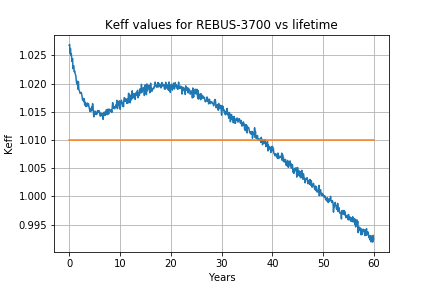
\includegraphics[scale=0.7]{./images/us/keff.png}
	\end{center}
	\caption{Change in $k_{eff}$ value in the REBUS-3700 core. The $k_{eff}$ drops below
		1.01 after 40 years of operation.}
	\label{fig:keff}
\end{figure}

\begin{figure}[htbp!]
	\begin{center}
		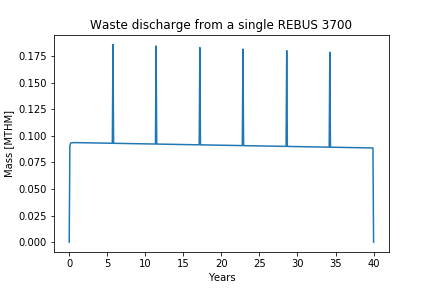
\includegraphics[scale=0.7]{./images/us/rebus_waste.png}
	\end{center}
	\caption{Mass of waste discharged from a single REBUS reactor. The peaks
		are due to the timestep differences in \Cyclus and SaltProc. \Cyclus
		uses 30.43 days for a month (1/12 of 365.25), and SaltProc uses 30-day
		timesteps. The peaks occur when two SaltProc timestep-worth of waste is discharged
		per one \Cyclus timestep.
	}
	\label{fig:rebus_waste}
\end{figure}

This database is generated to demonstrate \gls{MSR} modeling capability in \Cyclus,
and there is a possibility for future benchmarking if other simulation tools are
applied to the topic.


\FloatBarrier


\section{Results}
Results show that the United States can transition into a
fully \gls{MSR} fleet, while reducing final repository
burden by reducing \gls{TRU} and depleted uranium
inventory.

\subsection{\gls{LWR} \gls{UNF} inventory}

Table \ref{tab:us_lwr_unf} lists the U.S. \gls{LWR} \gls{UNF} inventory
results in the simulation.
Since major deployment of \glspl{MSR} does not begin until 2110,
the U.S. has a long time to prepare and accumulate the \glspl{TRU}
required for \gls{MSR} fuel salt fabrication. The U.S. accumulates
an additional $196,976$ \gls{MTHM} of \gls{LWR} \gls{UNF}
from 2013 to 2130, the year when the last \gls{LWR} decommissions.
Figure \ref{fig:us_lwr_unf} shows the accumulation of \gls{LWR} \gls{UNF}.
This figure does not subtract the \gls{LWR} \gls{UNF} reprocessed.


\begin{figure}[htbp!]
	\begin{center}
		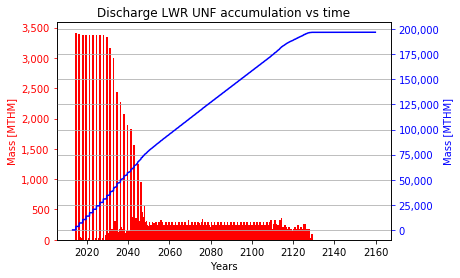
\includegraphics[scale=0.7]{./images/us/us_lwr_unf.png}
	\end{center}
	\caption{The cumulative mass of U.S. \gls{LWR} \gls{UNF}. The red bars are the
			mass discharged per timestep, and the blue line is the cumulative
			inventory. The large discharge quantity prior to 2040 is because the legacy \glspl{LWR}
			are deployed in the first timestep, thus discharging their fuel in sync.
			The later deployed \glspl{LWR} are not in sync, which makes the monthly
			discharge values more averaged out.}
	\label{fig:us_lwr_unf}
\end{figure}

\begin{table}[h]
	\centering
	\caption{U.S. \gls{LWR} \gls{UNF} material flow and inventory}
	\begin{tabular}{lrl}
		\hline
		\textbf{Category} & \textbf{Value [MTHM]} \\
		\hline
		US \gls{UNF} UOX generated in 2013-2050 & 78,281 \\
		US legacy \gls{LWR} \gls{UNF} in 2013 & 68,072 \\
		Total US \gls{LWR} \gls{UNF} inventory in 2050 & 146,353 \\
		Total US \gls{LWR} \gls{UNF} created from 2013 & 196,976 \\
		Total US \gls{LWR} \gls{UNF} created in U.S. & 265,048 \\
		\hline
	\end{tabular}
	\label{tab:us_lwr_unf}
\end{table}


\subsection{Reprocessing and fabrication material flow}

Metrics for \gls{LWR} \gls{UNF} reprocessing
are shown in table \ref{tab:us_rep}. A total of
$19,015$ MTHM of fuel salt is sent to \glspl{MSR}.
A total of $134,927$ MTHM of \gls{LWR} \gls{UNF}
are reprocessed to extract the \gls{TRU} for the fuel.

Figure \ref{fig:lwr_unf_reproc} shows the cumulative quantity of \gls{LWR}
\gls{UNF} reprocessed over time. The initial stage (2050-2100) is characterized
by a small amount of reprocessing due to the small number of \glspl{MSR} deployed.
From 2100, aggressive deployment of \glspl{MSR} causes
a large increase in the amount of \gls{LWR} \gls{UNF} reprocessed. This sudden
jump in demand of fuel salt is mediated by reprocessing the \gls{LWR} \gls{UNF} beforehand.

\begin{table}[h]
	\centering
	\caption{U.S. reprocessing metrics}
	\begin{tabular}{lS}
		\hline
		\textbf{Category} & \textbf{Value [MTHM]} \\
		\hline
		Total fuel salt mass sent to \gls{MSR}s & 19,015 \\
		Total TRU extracted from \gls{LWR} \gls{UNF} & 1,815 \\
		Total \gls{LWR} \gls{UNF} reprocessed & 134,927 \\
		Average monthly reprocessing demand of \gls{LWR} \gls{UNF} & 94.15 \\
		Average monthly fabrication of fuel salt & 13.26 \\
		Total raffinate stockpile & 4,024 \\
		\hline
	\end{tabular}
	\label{tab:us_rep}
\end{table}


\begin{figure}[htbp!]
	\begin{center}
		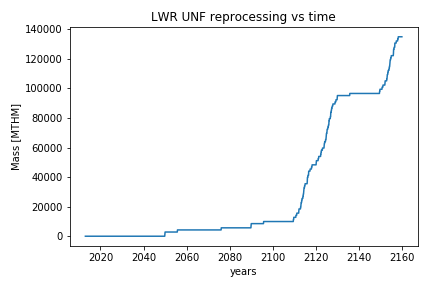
\includegraphics[scale=0.7]{./images/us/lwr_unf_reproc.png}
	\end{center}
	\caption{The Cumulative mass of \gls{LWR} \gls{UNF} reprocessed for \gls{MSR} salt fabrication.}
	\label{fig:lwr_unf_reproc}
\end{figure}

\subsection{Waste inventory and resource usage}

Table \ref{tab:us_waste} shows the masses of various nuclear waste
inventories at the end of the simulation. Large quantities of \gls{LWR}
\gls{UNF} ($132,094$ MTHM) and depleted uranium ($~1.1$ million tons)
remain unused, meaning that more \glspl{MSR} could have been deployed.
The tails usage from the \glspl{MSR} is not significant compared to
the quantity of tails accumulated ($~0.2\%$ of the total tails inventory).
One way to use more tails
is to substitute depleted uranium for initial
fuel salt fabrication. This would mean increasing the \gls{TRU} composition
in the fuel salt to make up for the decrease in $^{235}U$, which is viable,
since there are still $132,094$ MTHM of \gls{LWR} \gls{UNF} leftover
to extract \gls{TRU} from.

Figure \ref{fig:msr_waste} shows the monthly discharge and cumulative
inventory of waste from \glspl{MSR}. The discharge mass increases with
\gls{MSR} deployment. The mass of depleted uranium sent to \glspl{MSR} coincides
with the waste outflux, since the mass in the \gls{MSR} is kept constant.

\begin{table}[h]
	\centering
	\caption{U.S. waste metrics.}
	\begin{tabular}{lrl}
		\hline
		\textbf{Category} & \textbf{Value [MTHM]} \\
		\hline
			\gls{LWR} \gls{UNF} leftover inventory & 130,120 \\
			Total waste from \gls{MSR}s & 2,972 \\
			Total tails created from 2013 & 1,192,722 \\
			Total reprocessed uranium stockpile & 260,867 \\
			Total tails used & 2,972 \\
			Total remaining tails inventory & 1,189,753 \\
			Total natural U used & 1,389,698 \\
		\hline
	\end{tabular}
	\label{tab:us_waste}
\end{table}


\begin{figure}[htbp!]
	\begin{center}
		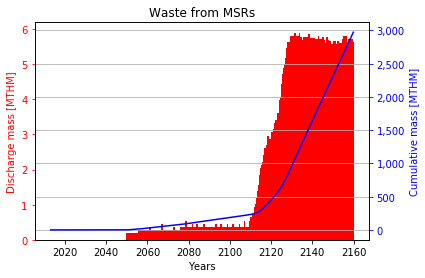
\includegraphics[scale=0.7]{./images/us/msr_waste.png}
	\end{center}
	\caption{Monthly discharged waste and cumulative waste inventory from
			\glspl{MSR}. The red bars are monthly discharge values, while
			the blue line is the cumulative quantity.}
	\label{fig:msr_waste}
\end{figure}


\section{Conclusion}
The United States can transition into a fully \gls{MSR} fleet with an
installed capacity of 100 GWe by 2130. With the deployment
scheme used in the simulation, the U.S. will have sufficient
time to prepare the fuel salt necessary for major \gls{MSR} deployment
beginning in 2110. Supporting the \gls{MSR} fleet requires an average
\gls{LWR} \gls{UNF} reprocessing capacity of $94.15$ MTHM per month, and an average fuel salt
fabrication capacity of $13.26$ MTHM per month. The reprocessing capacity demand is similar to the
current capacity of the La Hague plant in France (91.6 MTHM per month) \cite{schneider_spent_2008}.

The deployment of the REBUS-3700 \gls{MSR} design allows a reduction
in final repository burden, by transmuting the \gls{TRU} and reducing depleted uranium inventory.
However, \gls{TRU} extraction requires more advanced reprocessing methods than the currently
widely-deployed PUREX method. Resource utilization can be improved if depleted
uranium is used instead of natural uranium to fabricate initial fuel, since
there is still more than one million tons of depleted uranium available at the
end of the simulation. This would require a higher \gls{TRU} concentration
in the fuel, which is plausible since $132,094$ MTHM of \gls{LWR} \gls{UNF}
are still available for reprocessing.

In reality, however, complications with \gls{TRU} vectors and changes in \gls{MSR}
performance will occur, due to variations in \gls{LWR} \gls{UNF}
cooling (decay) time and discharge burnup. This would require careful fabrication of the initial fuel salt
so that the desired reactor parameters - multiplication factor, power density - are achieved. Another
challenge of this transition scenario is the aggressive build rates, which is not
considered in this work.

In conclusion, the U.S. can reduce its waste inventory by transitioning into
burner \glspl{MSR}. Choosing a U-Pu cycle instead of a Th-$^{233}U$ cycle
eliminates the need to introduce new resources (thorium), usage of moderators,
and allows utilization of depleted uranium, which would otherwise be waste.
Fissile (separated \gls{TRU}) and fertile (depleted uranium) material are
not limiting factors in the simulation, and a large inventory of \gls{LWR} \gls{UNF}
and depleted uranium remained at the end of the simulation.
